% !TeX root = ../main.tex
\section{Favorita販売データへの適用}
\label{sec:application}
\subsection{分析目的とデータ}
エクアドルの小売企業Corporación Favoritaの販売データ\citep{favoritadata}を用いる。訓練中に全12カテゴリの正販売日の割合が\(80\%\)以上で、各系列に変動がある店舗のうち最小番号の店舗1（Quito）を選んだ。対象カテゴリは図\ref{fig:favorita-mse}に示す。

2016年7月1日から2017年2月28日を訓練、2017年3月1日から4月30日を検証、5月1日から8月15日をテストとする。欠測の2016年12月25日は補間せず、7日ラグの窓全体が観測される場合のみ用いる。訓練は欠測前後で区切り、検証61時点、テスト107時点を評価する。

販売量を\(y_{j,t}\)、曜日を\(d(t)\)として、入力を
\begin{equation}
 x_{j,t}=\frac{\log(1+y_{j,t})-m_{j,d(t)}}{s_j}
 \label{eq:favorita-transform}
\end{equation}
へ変換する。\(m_{j,d}\)は訓練区間における曜日別の対数販売量の平均、\(s_j\)は曜日平均を除いた訓練残差の標準偏差である。訓練で求めた変換を検証・テストに固定し、外生変数は入力しない。

\subsection{候補設定と検証による選択}
GSE-VAR、NGCのcMLP\citep{tank2022}、線形VAR(SGL)を比較し、最大ラグを7日とする。GSE-VARは隠れ層1層・幅8、平滑化係数\(0.01\)、重み減衰\(0.001\)、初期選択確率\(0.5\)とする。尺度\(s\in\{0,0.3,1,2,3,4,6,10,20,40\}\)を\(\lambda_0=s/(7\times12^2)\)に換算し、係数・ゲート学習率の組\((0.003,0.03),(0.001,0.01),(0.001,0.03)\)と合わせて30候補を比較する。cMLPは隠れ層1層・幅100、L2係数\(0.01\)とし、階層グループ正則化係数\(\{0,0.001,0.003,0.01,0.03,0.1,0.3,0.5,1,10\}\)と学習率\(\{0.01,0.003\}\)の20候補を近接勾配法で学習する。両ニューラルモデルは最大5000エポック、初期200エポックまでは20、その後は100エポックごとに検証する。線形VARはL1係数\(10^{-4}\)、グループ係数\(\{0,10^{-5},3\times10^{-5},10^{-4},3\times10^{-4},10^{-3},0.003,0.01,0.03,0.1\}\)の10候補とする。検証MSE最小の候補・チェックポイントを採用し、同点ではエポック数、候補番号の順で選ぶ。

採用されたGSE-VARは\(s=2\)、学習率の組\((0.003,0.03)\)、1400エポック、cMLPは正則化係数\(0.1\)、学習率\(0.01\)、5000エポックであり、線形VARのグループ係数は\(0.01\)であった。検証最良モデルを再推定せずテストで評価する。学習初期値は42とする。

\subsection{予測誤差と選択構造}
目的変数\(j\)のテストMSEと、全変数をまとめたMSEを
\begin{equation}
 \mathrm{MSE}_j=\frac{1}{N_{\mathrm{test}}}\sum_t(\widehat x_{j,t}-x_{j,t})^2,
 \qquad
 \mathrm{MSE}=\frac{1}{12}\sum_{j=1}^{12}\mathrm{MSE}_j
 \label{eq:favorita-mse}
\end{equation}
と定める。全体のRMSEは\(\sqrt{\mathrm{MSE}}\)である。表\ref{tab:favorita-overall}のとおり、GSE-VAR、cMLP、線形VARのテストMSEはそれぞれ\(0.4620,0.4727,0.4703\)、ラグを統合した非自己辺数は7本、39本、66本であった。GSE-VARは三手法の中で最も低いテストMSEと少ない選択辺数を示した。

\begin{table}[!htbp]
\centering\small
\caption{Favoritaのモデル選択とテスト評価。誤差は標準化尺度、辺数は自己辺を除く。各手法1モデルの値である。}
\label{tab:favorita-overall}
\begin{tabular}{lrrrr}
\toprule
手法&検証MSE&テストMSE&テストRMSE&非自己辺数\\
\midrule
GSE-VAR&0.4533&0.4620&0.6797&7\\
cMLP&0.4617&0.4727&0.6875&39\\
線形VAR(SGL)&0.4810&0.4703&0.6858&66\\
\bottomrule
\end{tabular}
\end{table}



図\ref{fig:favorita-mse}では調理済食品と魚介の誤差が大きい。GSE-VARは酒類で線形VARより低いMSEを示す一方、冷凍食品では線形VARが低い。

\begin{figure}[!htbp]
\centering
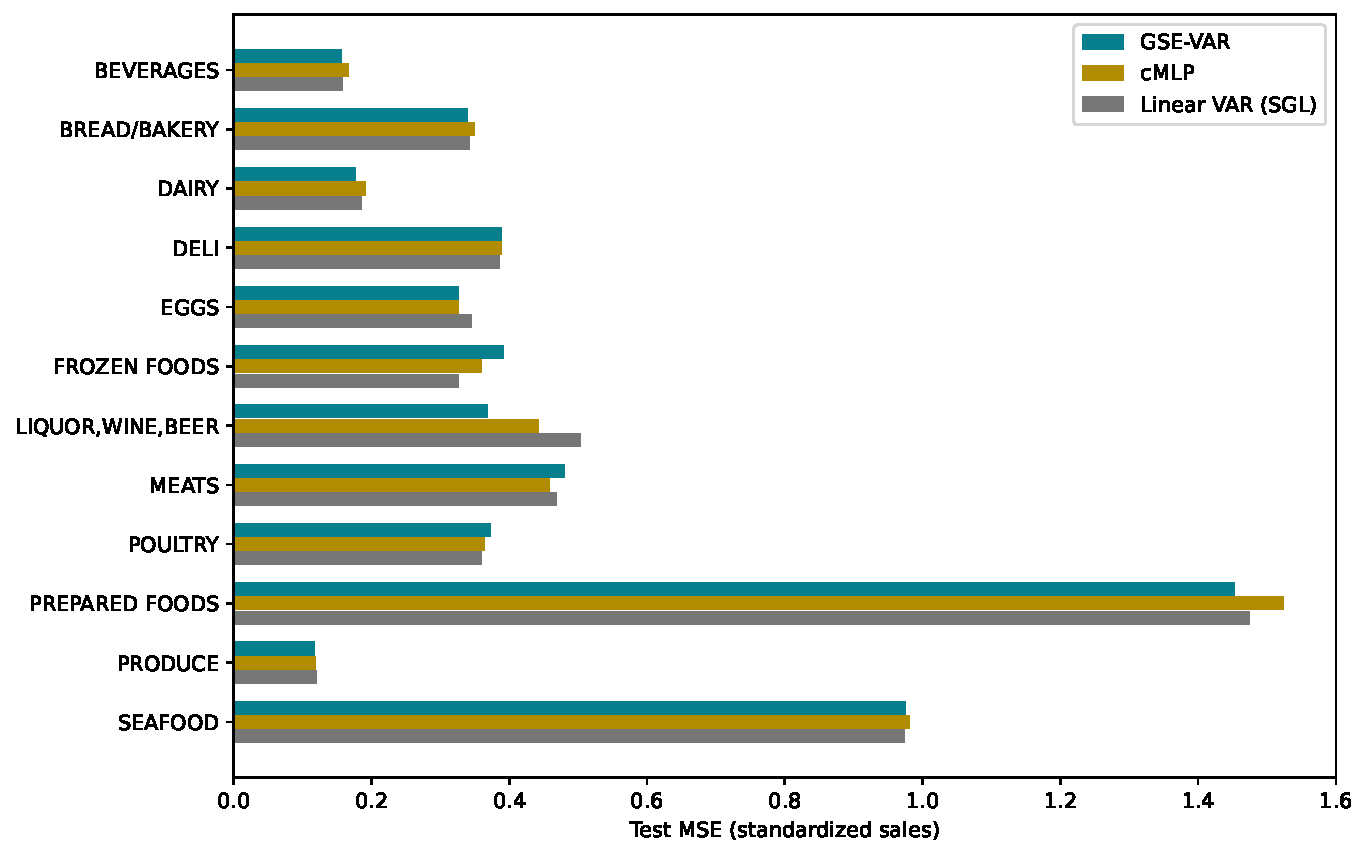
\includegraphics[width=.94\linewidth]{figures/favorita_target_mse.pdf}
\caption{目的変数別テストMSE。三手法で同一の107時点を評価し、曜日調整した対数販売量の標準化尺度で比較する。}
\label{fig:favorita-mse}
\end{figure}

\subsection{カテゴリ間の関係の記述}
図\ref{fig:favorita-structures}に三手法の選択構造、図\ref{fig:favorita-links}にGSE-VARの7本の非自己選択経路を示す。GSE-VARの各辺はいずれも一つのラグで構成され、モデル内で利用可能な予測経路を表す。

\begin{figure}[H]
\centering
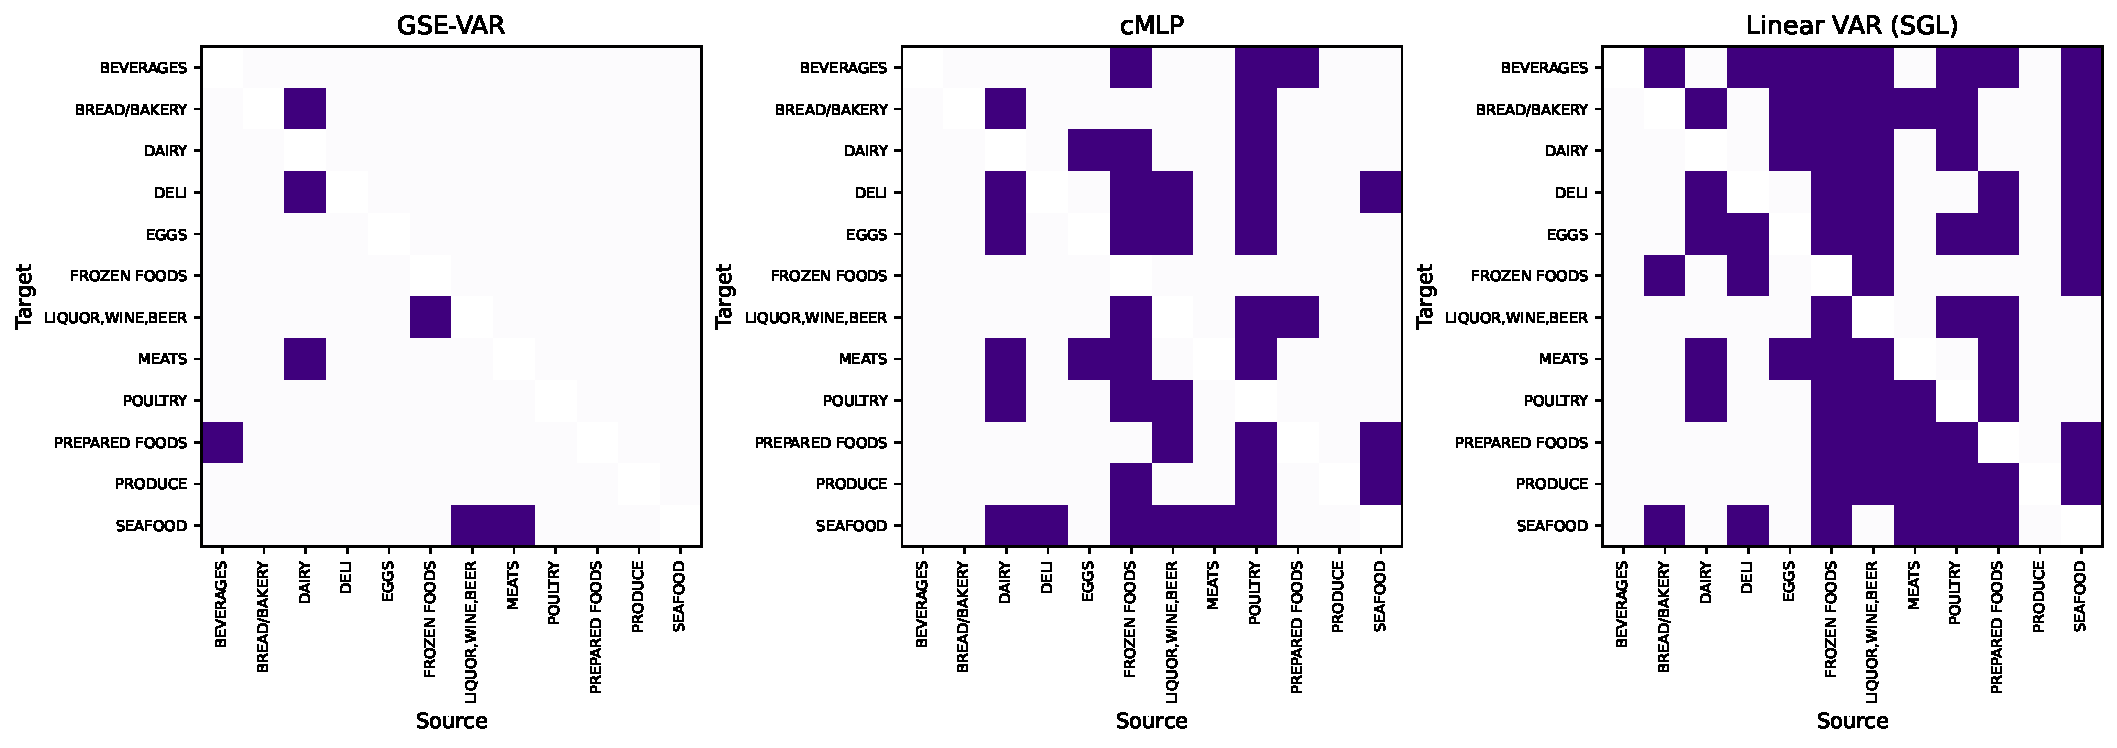
\includegraphics[width=\linewidth]{figures/favorita_structures.pdf}
\caption{Favoritaのラグ統合選択構造。左からGSE-VAR、cMLP、線形VAR。行が予測対象、列が入力で、紫色は少なくとも一つのラグが選択された変数対を示す。cMLPは入力層の非零重み、線形VARは非零係数から辺を抽出し、自己辺は表示から除いた。}
\label{fig:favorita-structures}
\end{figure}

係数の符号はテスト時点の\(80\%\)以上で正なら正、\(80\%\)以上で負なら負、他は混在とする。酒類から魚介は混在、残る6経路は正であった。

\begin{figure}[H]
\centering
\resizebox{\linewidth}{!}{\begin{tikzpicture}[box/.style={draw=violet!80!black,fill=violet!5,rounded corners=2pt,minimum width=3.1cm,minimum height=.65cm,font=\small},route/.style={-{Stealth[length=2.5mm]},line width=.9pt,draw=violet!80!black},every edge quotes/.style={font=\footnotesize}]
\node[box] (dairy) at (-4,2.2) {乳製品};
\node[box] (bread) at (0.3,3.2) {パン・ベーカリー};
\node[box] (deli) at (0.3,1.9) {デリ食品};
\node[box] (meat) at (0.3,0.6) {肉類};
\node[box] (seafood) at (5,0.6) {魚介};
\node[box] (frozen) at (-4,-1) {冷凍食品};
\node[box] (liquor) at (0.3,-1) {酒類};
\node[box] (beverages) at (-4,-2.5) {飲料};
\node[box] (prepared) at (5,-2.5) {調理済食品};
\draw[route] (beverages.east) -- node[above,font=\footnotesize,fill=white,inner sep=1pt,text=violet!80!black] {\(+0.361\)（7日前）} (prepared.west);
\draw[route] (dairy.east) -- node[above,font=\footnotesize,fill=white,inner sep=1pt,text=violet!80!black] {\(+0.306\)} (bread.west);
\draw[route] (dairy.east) -- node[below,font=\footnotesize,fill=white,inner sep=1pt,text=violet!80!black] {\(+0.437\)} (deli.west);
\draw[route] (frozen.east) -- node[above,font=\footnotesize,fill=white,inner sep=1pt,text=violet!80!black] {\(+0.146\)} (liquor.west);
\draw[route] (dairy.south east) -- node[below,sloped,font=\footnotesize,fill=white,inner sep=1pt,text=violet!80!black] {\(+0.369\)} (meat.north west);
\draw[route,dashed,draw=gray] (liquor.east) -- node[below,sloped,font=\footnotesize,fill=white,inner sep=1pt,text=gray] {\(+0.035\)} (seafood.south west);
\draw[route] (meat.east) -- node[above,font=\footnotesize,fill=white,inner sep=1pt,text=violet!80!black] {\(+0.233\)} (seafood.west);
\end{tikzpicture}
}
\caption{GSE-VARの非自己選択経路。矢印は入力から予測対象への向きを示す。数値は標準化尺度の107テスト時点における係数の中央値。飲料から調理済食品は7日前、他は1日前の入力であり、破線は符号が混在する経路を表す。}
\label{fig:favorita-links}
\end{figure}

係数は予測式上の重みを表す。図\ref{fig:favorita-links}のように、カテゴリ名・ラグ・係数を組み合わせることで、予測を担う経路を具体的に検討できる。局所感度との対応には式\eqref{eq:jacobian}を用い、共通する購買動向や販促の影響は第\ref{sec:limitations}節の課題として扱う。
